% !TeX root = ../main.tex
% Add the above to each chapter to make compiling the PDF easier in some editors.

\chapter{Background}\label{chapter:background}

\section{Dynamic Programming vs. Greedy}
Many algorithmic problems involve selecting a sequence of decisions that together optimize a global objective. Two widely used approaches for solving such problems are greedy algorithms and dynamic programming (DP). While both aim to construct efficient solutions, they differ fundamentally in how they explore the solution space and reason about optimality.
\subsection{Greedy Algorithms}
Greedy algorithms build a solution incrementally by making locally optimal decisions at each step. At every stage, the algorithm selects the option that appears best according to a predefined heuristic, without reconsidering previous choices. This strategy is attractive due to its simplicity, low computational overhead, and ease of implementation.

Greedy approaches are particularly effective when a problem exhibits the greedy-choice property, meaning that a locally optimal decision can be shown to lead to a globally optimal solution.
\newline

\sparagraph{Example.} An easy example illustrating the greedy-choice property is the problem where we are given a sequence of distinct numbers and we want to take a subset of $K$ numbers with the goal of maximizing the sum of those numbers. The intuitive and correct way to choose the numbers is by selecting the largest $K$ numbers of the sequence for the subset (denoted by $S$).
We can prove this by contradiction: suppose there is an optimal solution where a number of the chosen subset does not belong to $S$, we can swap that number with an unchosen number of the set $S$ and we would have a strictly better solution, which leads to contradiction.
\newline

\noindent
Despite this limitation, greedy algorithms are frequently used in performance-critical systems where execution speed and simplicity are prioritized over absolute optimality.

\subsection{Dynamic Programming}

Dynamic programming (DP) addresses optimization problems by systematically exploring all relevant subproblems and combining their solutions to obtain a globally optimal result. The core idea is to decompose a problem into overlapping subproblems, solve each subproblem once, and store its result to avoid redundant computation.

Unlike greedy algorithms, dynamic programming evaluates the long-term consequences of decisions. By considering multiple possible choices at each stage and selecting the one that minimizes or maximizes a well-defined cost function, DP can guarantee optimality when the problem satisfies optimal substructure and overlapping subproblems.

%formal definitiotn of knapsack DP 
\begin{comment}
We define the 0/1 Knapsack problem formally as follows: there are $n$ items where each item $i$ has value $v_i$ and weight $w_i$ and the knapsack capacity is $W$. We need to choose a subset of items that fits the capacity while maximizing the total value.
Define the DP table: $dp[i][c] =$ maximum value achievable using the first $i$ items with capacity $c$. So the result is stored in $dp[n][W]$.
The base cases are $dp[i][0] = 0$ for all $i$ and $dp[0][c] = 0$ for all $c$. The recurrence is defined for each item $i$ and capacity $c$ as follows:
If $w_i > c$ (item does not fit): $dp[i][c] = dp[i - 1][c]$. 
Otherwise choose best of taking or not taking the item: $dp[i][c] = \max(dp[i - 1][c], dp[i - 1][c - w_i] + v_i)$.
Time complexity is $O(nW)$.
\end{comment}

The primary trade-off of dynamic programming is computational complexity. DP solutions often require more time and memory than greedy alternatives, especially when the state space is large. As a result, practical DP implementations frequently rely on carefully designed cost models, state compression, or bounded problem sizes to remain efficient.

\section{Data Structures}
Efficient algorithmic design relies not only on the choice of optimization strategy but also on the use of appropriate data structures. This section introduces the two core data structures used throughout this thesis: max heaps and tries. Both play an important role in managing candidates and efficiently representing string data.

\subsection{Max Heap}
A max heap is a complete binary tree-based data structure that maintains the heap property: the key of each node is greater than or equal to the keys of its children. As a result, the maximum element is always stored at the root of the heap.

The primary operations supported by a max heap include insertion, extraction of the maximum element, and key updates. Each of these operations can be performed in logarithmic time with respect to the number of elements in the heap. This efficiency makes max heaps particularly well suited for priority-based selection tasks, where the most valuable or promising element must be accessed repeatedly.
\clearpage


\begin{figure}[h]
  \centering
  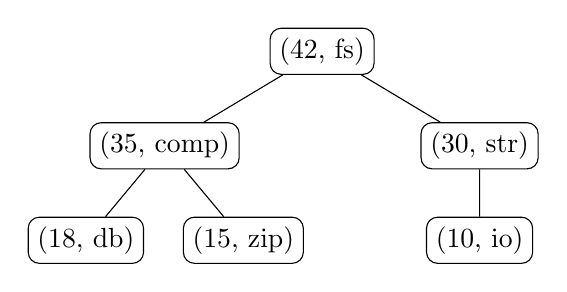
\begin{tikzpicture}[
    level distance=1.2cm,
    level 1/.style={sibling distance=4cm},
    level 2/.style={sibling distance=2cm},
    every node/.style={draw, rectangle, rounded corners, align=center}
    ]
    
    \node {(42, fs)}
    child {node {(35, comp)}
    child {node {(18, db)}}
    child {node {(15, zip)}}
    }
    child {node {(30, str)}
    child {node {(10, io)}}
    };
    
  \end{tikzpicture}
  \caption{Initial max heap.}
  \label{maxheap-initial}
\end{figure}

\sparagraph{Example.} The max heap from the example above stores the following data: \{(42, ``fs''), (35, ``comp''), (30, ``str''), (18, ``db''), (15, ``zip''), (10, ``io'')\}. These (int, string) pairs can represent gains and symbols respectively in the context of FSST, where the gain is a heuristic to measure how good a symbol is. Storing the information in this format allows for the symbol with the highest gain to be selected first from the max heap with the 'pop' operation, extracting the element in the root node.   

As the figure shows, each node has a higher key than its children. In this case the key comparison occurs between the integers (the first element of the pair) then between the strings in case of a tie. 

\begin{figure}[h]
\centering
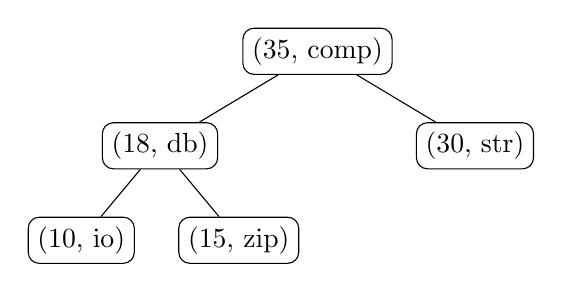
\begin{tikzpicture}[
  level distance=1.2cm,
  level 1/.style={sibling distance=4cm},
  level 2/.style={sibling distance=2cm},
  every node/.style={draw, rectangle, rounded corners, align=center}
]

\node {(35, comp)}
  child {node {(18, db)}
    child {node {(10, io)}}
    child {node {(15, zip)}}
  }
  child {node {(30, str)}};

\end{tikzpicture}
\caption{Max heap after pop operation.}
\label{maxheap-pop}
\end{figure}

The pop operation extracts the element of the root node, which is the element with the highest key. Then the rest of the elements are reordered to maintain the max heap property. This operation has a runtime complexity of $O(\log(n))$, where $n$ is the number of nodes in the heap.  

\begin{figure}[h]
\centering
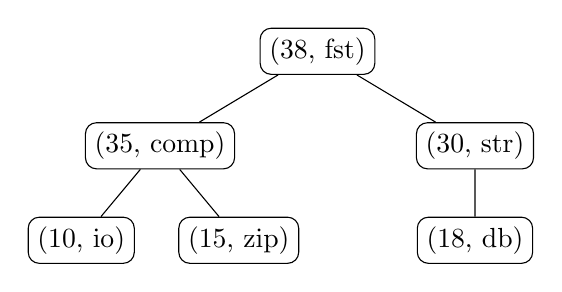
\begin{tikzpicture}[
  level distance=1.2cm,
  level 1/.style={sibling distance=4cm},
  level 2/.style={sibling distance=2cm},
  every node/.style={draw, rectangle, rounded corners, align=center}
]

\node {(38, fst)}
  child {node {(35, comp)}
    child {node {(10, io)}}
    child {node {(15, zip)}}
  }
  child {node {(30, str)}
    child {node {(18, db)}}
  };

\end{tikzpicture}
\caption{Max heap after inserting the element (38, fst).}
\label{maxheap-insert}
\end{figure}

The insert operation inserts a new element to the heap and then reorders the rest of the elements to maintain the max heap property like in the pop operation. This operation also has a runtime complexity of $O(\log(n))$.
\newline

\noindent
In the context of algorithmic optimization, max heaps are often used to manage candidate sets ordered by a score or heuristic value. They enable fast retrieval of the currently best candidate while allowing dynamic updates as new candidates are generated or existing ones are reweighted.

\subsection{Trie}
A trie, also known as a prefix tree, is a tree-based data structure used to store and retrieve strings efficiently by exploiting their shared prefixes. Each node in a trie represents a prefix of one or more strings, and edges correspond to individual characters or bytes. Strings are represented by paths from the root to terminal nodes which can also store other data related to the strings (like mappings).

Tries provide efficient operations for prefix-based queries, insertion, and lookup, all of which can be performed in time proportional to the length of the string rather than the number of stored strings. This makes them particularly suitable for applications involving multiple search operations for strings with commun prefixes.


\begin{figure}[h]
  \centering
  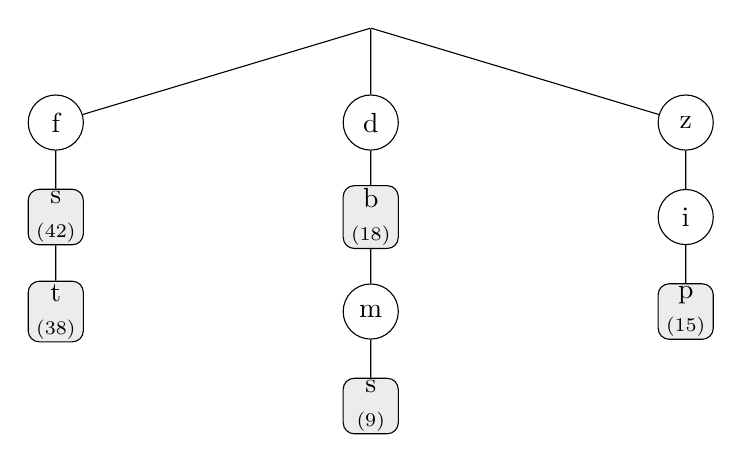
\begin{tikzpicture}[
    level distance=1.2cm,
    level 1/.style={sibling distance=4cm},
    level 2/.style={sibling distance=2cm},
    level 3/.style={sibling distance=1.5cm},
    every node/.style={draw, circle, minimum size=7mm, inner sep=1pt, align=center},
    terminal/.style={shape=rectangle, draw, rounded corners, fill=gray!15, align=center}
    ]
    \node[draw=none, inner sep=0, minimum size=0] {} % root
    child {node {f}
    child {node[terminal] {s\\\scriptsize(42)}
    child {node[terminal] {t\\\scriptsize(38)}}
    }
    }
    child {node {d}
    child {node[terminal] {b\\\scriptsize(18)}
    child {node {m}
    child {node[terminal] {s\\\scriptsize(9)}}
    }
    }
    }
    child {node {z}
    child {node {i}
    child {node[terminal] {p\\\scriptsize(15)}}
    }
    };
  \end{tikzpicture}
  \caption{Example trie storing short strings.}
  \label{trie-example}
\end{figure}

\sparagraph{Example.} The trie from the example above stores the 5 strings ``fs'', ``fst'', ``db'', ``dbms'', and ``zip'' with a mapping for each string as an integer stored in the corresponding terminal node. The strings stored can be interpreted as the symbols of a symbol table and the integers as the corresponding codes (one code for each symbol) in the context of FSST. Details will follow in next sections.

As the trie shows, terminal nodes (gray nodes) mark the end of a symbol and contain the corresponding code. A symbol can be searched by a traversal of the trie from the root to the terminal node. Each edge corresponds to the next character in the symbol search.

Symbols can have other symbols as a prefix and in that case the terminal node of the prefix symbol will be an ancestor of the terminal node of the bigger symbol. For example, the trie above stores the symbol ``db'' which is a prefix of the symbol ``dbms''.


\begin{comment}
Citation test~\parencite{latex}.

Acronyms must be added in \texttt{main.tex} and are referenced using macros. The first occurrence is automatically replaced with the long version of the acronym, while all subsequent usages use the abbreviation.

E.g. \texttt{\textbackslash ac\{TUM\}, \textbackslash ac\{TUM\}} $\Rightarrow$ \ac{TUM}, \ac{TUM}

For more details, see the documentation of the \texttt{acronym} package\footnote{\url{https://ctan.org/pkg/acronym}}.
\subsection{Subsection}

See~\autoref{tab:sample}, \autoref{fig:sample-drawing}, \autoref{fig:sample-plot}, \autoref{fig:sample-listing}.

\begin{table}[htpb]
  \caption[Example table]{An example for a simple table.}\label{tab:sample}
  \centering
  \begin{tabular}{l l l l}
    \toprule
      A & B & C & D \\
    \midrule
      1 & 2 & 1 & 2 \\
      2 & 3 & 2 & 3 \\
    \bottomrule
  \end{tabular}
\end{table}

\begin{figure}[htpb]
  \centering
  % This should probably go into a file in figures/
  \begin{tikzpicture}[node distance=3cm]
    \node (R0) {$R_1$};
    \node (R1) [right of=R0] {$R_2$};
    \node (R2) [below of=R1] {$R_4$};
    \node (R3) [below of=R0] {$R_3$};
    \node (R4) [right of=R1] {$R_5$};

    \path[every node]
      (R0) edge (R1)
      (R0) edge (R3)
      (R3) edge (R2)
      (R2) edge (R1)
      (R1) edge (R4);
  \end{tikzpicture}
  \caption[Example drawing]{An example for a simple drawing.}\label{fig:sample-drawing}
\end{figure}

\begin{figure}[htpb]
  \centering

  \pgfplotstableset{col sep=&, row sep=\\}
  % This should probably go into a file in data/
  \pgfplotstableread{
    a & b    \\
    1 & 1000 \\
    2 & 1500 \\
    3 & 1600 \\
  }\exampleA
  \pgfplotstableread{
    a & b    \\
    1 & 1200 \\
    2 & 800 \\
    3 & 1400 \\
  }\exampleB
  % This should probably go into a file in figures/
  \begin{tikzpicture}
    \begin{axis}[
        ymin=0,
        legend style={legend pos=south east},
        grid,
        thick,
        ylabel=Y,
        xlabel=X
      ]
      \addplot table[x=a, y=b]{\exampleA};
      \addlegendentry{Example A}
      \addplot table[x=a, y=b]{\exampleB};
      \addlegendentry{Example B}
    \end{axis}
  \end{tikzpicture}
  \caption[Example plot]{An example for a simple plot.}\label{fig:sample-plot}
\end{figure}

\begin{figure}[htpb]
  \centering
  \begin{tabular}{c}
  \begin{lstlisting}[language=SQL]
    SELECT * FROM tbl WHERE tbl.str = str
  \end{lstlisting}
  \end{tabular}
  \caption[Example listing]{An example for a source code listing.}\label{fig:sample-listing}
\end{figure}
\end{comment}